%Template Proposal PI/Magang
%Departemen Teknik Elektro dan Informatika
%Sekolah Vokasi UGM

%Dikembangkan oleh Dr. Fahmizal, S.T., M.Sc. dan Tim

%Perangkat lunak yang digunakan untuk mengolah LaTEX pada template ini adalah
%- TeXstudio
%- MiKTex
%- Overleaf (LaTEX editor berbasis daring)


\documentclass[12pt, a4paper, onecolumn, oneside, final]{report}

%Isi identitas proyek akhir disini

\providecommand{\tipe}{Proposal Praktik Industri/Magang MBKM}
\providecommand{\permohonan}{Proposal Permohonan Praktik Industri atau MBKM}

\providecommand{\perusahaan}{PT. xxx}
\providecommand{\alamatPerusahaan}{Alamat Perusahaan}
\providecommand{\websitePerusahaan}{https://otomasi.sv.ugm.ac.id/}

\providecommand{\penulisPertama}{Amelia Dwi Widyawati} 
\providecommand{\penulisKedua}{Tasya Wulandari} 
\providecommand{\nimPertama}{XX/XXXXXX/SV/XXXXX}
\providecommand{\nimKedua}{XX/XXXXXX/SV/XXXXX}

\providecommand{\prodi}{Teknologi Rekayasa Elektro} 
\providecommand{\departemen}{Departemen Teknik Elektro dan Informatika}
\providecommand{\fakultas}{Sekolah Vokasi}
\providecommand{\universitas}{Universitas Gadjah Mada} 

\providecommand{\tglpengesahan}{\today} 
\providecommand{\tglpersetujuan}{\today}
\providecommand{\tglpernyataan}{\today}
\providecommand{\tahun}{\the\year{}} 

\providecommand{\waktuPelaksanaan}{(Tanggal mulai) -  (Tanggal selesai) (Tahun) ((Jumlah Minggu))} 

\providecommand{\dosenPembimbing}{Dr. Fahmizal, S.T., M.Sc.} 
\providecommand{\koorprodi}{Dr. Fahmizal, S.T., M.Sc.} 
\providecommand{\pembimbing}{Dr. Fahmizal, S.T., M.Sc.} 
\providecommand{\nikaPembimbing}{111198807201609101}
\providecommand{\NIPkoorprodi}{111198807201609101} %
\providecommand{\NIPpembimbing}{111198807201609101} 

% Mengatur bahasa latex
\usepackage[indonesian]{babel}
\usepackage[utf8]{inputenc}

% Untuk pengaturan spacing
\usepackage{setspace}
\onehalfspacing

% Untuk mengatur level section 
\setcounter{secnumdepth}{6}

% Digunakan untuk memasukan gambar ke laporan. 
\usepackage{graphicx}
\graphicspath{{gambar/}}
\usepackage{float}
\usepackage[hang,centerlast, nooneline ,small,md]{subfigure}
\usepackage[subfigure]{tocloft}

% Untuk mengatur spacing antara paragraf
\usepackage{parskip}

% Membuat indent
\usepackage{indentfirst}
\setlength\parindent{1cm}

% Untuk mengkustomisasi margin
\usepackage{scrextend}

% Untuk mengatur header dan footer
\usepackage{fancyhdr}

% Membuat seluruh tulisan menjadi Times New Roman. 
% \usepackage{pslatex}

% Merubah numbering chapter dan section untuk judul setiap bab menggunakan romawi dan judul anak bab menggunakan arabic
\renewcommand{\thesection}{\arabic{chapter}.\arabic{section}\hspace{0.05cm}}
\renewcommand{\thesubsection}{\arabic{chapter}.\arabic{section}.\arabic{subsection}\hspace{-0.25cm}}
\renewcommand{\thesubsubsection}{\Alph{subsubsection}.\hspace{-0,25cm}}

% Mengatur identasi judul section dan subsection
%\titleformat{\section}[block]{\bfseries}{\thesection.}{1em}{}
%\titleformat{\subsection}[block]{\hspace{2em}}{\thesubsection}{1em}{}

% Merubah huruf kapital pada judul daftar isi, daftar gambar, dan daftar table
\usepackage{tocloft}
\renewcommand{\cfttoctitlefont}{\hfil\large\bfseries\MakeUppercase}
\renewcommand{\cftloftitlefont}{\hfil\large\bfseries\MakeUppercase}
\renewcommand{\cftlottitlefont}{\hfil\large\bfseries\MakeUppercase}

\renewcommand\cftchappresnum{BAB }
\renewcommand\cftchapaftersnum{}
\newlength\mylen
\settowidth\mylen{\bfseries BAB 1 :\ } % if more than 9 chapters, use "Chapter 10"
\cftsetindents{chap}{0pt}{\mylen}

% Mengatur font section
\usepackage{sectsty}
\sectionfont{\fontsize{12}{14}\selectfont}
\subsectionfont{\fontsize{12}{14}\selectfont}
\subsubsectionfont{\fontsize{12}{14}\selectfont}

% Untuk merupakan format penulisan BAB
\usepackage{titlesec}
\titleformat{\chapter}
{\doublespacing\fontsize{14pt}{16pt}\bfseries}
{\MakeUppercase{\chaptertitlename\ \Roman{chapter}}\filcenter}
{0.15cm}{\centering\uppercase}
\titlespacing*{\chapter}{0pt}{-1cm}{20pt}

% Mengatur spacing section
\titlespacing*{\section}
{0pt}{10pt}{0cm}
\titlespacing*{\subsection}
{0pt}{10pt}{0cm}
\titlespacing*{\subsubsection}
{0pt}{10pt}{0cm}

% Digunakan untuk mengatur caption dalam dokumen.
\usepackage[font=footnotesize,format=plain,labelfont=bf,up,textfont=up]{caption}

% Untuk menghapus titik dua (colon)
\captionsetup[figure]{labelsep=space}
\captionsetup[table]{labelsep=space}

% Mengatur nomor caption gambar
\renewcommand{\thefigure}{\arabic{chapter}.\arabic{figure}}

% Mengatur nomor caption table
\renewcommand{\thetable}{\arabic{chapter}.\arabic{table}}

% Mengatur Hyphenation pada latex
\tolerance=1
\emergencystretch=\maxdimen
\hyphenpenalty=10000
\hbadness=10000

% Untuk mengatur setting indent
\setlength\parindent{1cm}

% Untuk memasukkan table
\usepackage{tabularx}
\usepackage{multirow}

% Untuk mengatur width
\usepackage{changepage}

% Menggatur setting halaman 
\usepackage{geometry}
\geometry{
    left=3cm,            % <-- you want to adjust this
    top=3cm,
    right=2.5cm,
    bottom=3cm,
}

% Teks testing
\usepackage{blindtext}
\usepackage{lipsum}

% Untuk mengatur subscript supscript
\usepackage{fixltx2e}

% Untuk formatting quote pada halaman motto
\usepackage{epigraph}

% Untuk mengatur wrap picture
\usepackage{wrapfig}

% Untuk notasi matematika
\usepackage{amsmath}
\usepackage{stmaryrd}
\usepackage{mathtools}



% untuk mengatur label nomor pada rumus
\renewcommand{\theequation}{\arabic{chapter}.\arabic{equation}}

% Untuk mengatur spacing daftar gambar
\newcommand*{\noaddvspace}{\renewcommand*{\addvspace}[1]{}}
\addtocontents{lof}{\protect\noaddvspace}

%Menambahkan sumber gambar
\usepackage{url}
\newcommand*{\putsource}[1]{%
	\textbf{\small{Sumber: }} \small{\url{#1}}
}

%untuk mengatur package include table in excel
% \usepackage{pgfplotstable}

% untuk mengatur landscape page
\usepackage{rotating}

%untuk mengubah page menjadi landscape
\usepackage{pdflscape}

% untuk list
\usepackage{enumitem}
\newenvironment{packed_enum}{
    \begin{enumerate}[leftmargin=1.5\parindent]
        \setlength{\itemsep}{0pt}
        \setlength{\parskip}{0pt}
        \setlength{\parsep}{0pt}
        }{\end{enumerate}}

\newenvironment{packed_item}{
    \begin{itemize}[leftmargin=1.5\parindent]
        \setlength{\itemsep}{0pt}
        \setlength{\parskip}{0pt}
        \setlength{\parsep}{0pt}
        }{\end{itemize}}

%paket untuk bibTex
\usepackage{cite}
\bibliographystyle{IEEEtran}
%\bibliographystyle{apalike}

%paket untuk mengembed kode dalam LaTeX
\usepackage{listings}
\lstset{
    basicstyle=\small,
    %basicstyle=\ttfamily,
    columns=fullflexible,
    frame=single,
}

%paket untuk tabel
\usepackage{longtable}
\usepackage[table,xcdraw]{xcolor}
\usepackage{tabularx}
\usepackage{multirow}

%paket untuk url
% \usepackage{hyperref}
\usepackage[hidelinks]{hyperref} %remove red boxes

% styling python
\usepackage{color}
\usepackage{listings}    
\usepackage{courier}

\definecolor{mygreen}{rgb}{0,0.6,0}
\definecolor{mygray}{rgb}{0.5,0.5,0.5}
\definecolor{mymauve}{rgb}{0.58,0,0.82}

\lstset{ %
  backgroundcolor=\color{white},   % choose the background color
  basicstyle=\footnotesize,        % size of fonts used for the code
  breaklines=true,                 % automatic line breaking only at whitespace
  captionpos=b,                    % sets the caption-position to bottom
  commentstyle=\color{mygreen},    % comment style
  escapeinside={\%*}{*)},          % if you want to add LaTeX within your code
  keywordstyle=\color{blue},       % keyword style
  stringstyle=\color{mymauve},     % string literal style
}

%styling Processing
\usepackage{verbatim}

%Define Colors
\definecolor{black}{RGB}{0,0,0}
\definecolor{gray}{RGB}{102,102,102}		%#666666
\definecolor{function}{RGB}{0,102,153}		%#006699 lightblue
\definecolor{lightgreen}{RGB}{102,153,0}	%#669900
\definecolor{bluegreen}{RGB}{51,153,126}	%#33997e
\definecolor{magenta}{RGB}{217,74,122}	%#d94a7a
\definecolor{orange}{RGB}{226,102,26}		%#e2661a
\definecolor{purple}{RGB}{125,71,147}		%#7d4793
\definecolor{green}{RGB}{113,138,98}		%#718a62

\lstdefinelanguage{Processing}{
	%keyword1&2&6
	morekeywords = [3]{abstract, break, class, continue, default, enum, extends, false, final, finally, implements, import, instanceof, interface, native, new, null, package, private, protected, public, static, strictfp, throws, transient, true, void, volatile, length, assert, case, return, super, this, throw},
	%keyword3
	morekeywords = [4]{catch, do, for, if, else, switch, synchronized, while, try},
	%keyword4
	morekeywords = [5]{width, height, pixelHeight, displayHeight, displayWidth, focused, frameCount, frameRate, key, keyCode, keyPressed, mouseButton, mousePressed, mouseX, mouseY, pixels, pixelWidth, pmouseX, pmouseY},
	%keyword5
	morekeywords = [6]{Array, ArrayList, Boolean, Byte, BufferedReader, Character, Class, Double, Float, Integer, HashMap, PrintWriter, String, StringBuffer, StringBuilder, Thread, boolean, byte, char, color, double, float, int, long, short, FloatDict, FloatList, IntDict, IntList, JSONArray, JSONObject, PFont, PGraphics, PImage, PShader, PShape, PVector, StringDict, StringList, Table, TableRow, XML},
	%literal2
	morekeywords = [7]{ADD, ALIGN_CENTER, ALIGN_LEFT, ALIGN_RIGHT, ALPHA, ALPHA_MASK, ALT, AMBIENT, ARC, ARROW, ARGB, BACKSPACE, BASELINE, BEVEL, BLEND, BLUE_MASK, BLUR, BOTTOM, BOX, BURN, CENTER, CHATTER, CHORD, CLAMP, CLICK, CLOSE, CMYK, CODED, COMPLAINT, COMPOSITE, COMPONENT, CONCAVE_POLYGON, CONTROL, CONVEX_POLYGON, CORNER, CORNERS, CROSS, CUSTOM, DARKEST, DEGREES, DEG_TO_RAD, DELETE, DIAMETER, DIFFERENCE, DIFFUSE, DILATE, DIRECTIONAL, DISABLE_ACCURATE_2D, DISABLE_DEPTH_MASK, DISABLE_DEPTH_SORT, DISABLE_DEPTH_TEST, DISABLE_NATIVE_FONTS, DISABLE_OPENGL_ERRORS, DISABLE_PURE_STROKE, DISABLE_TEXTURE_MIPMAPS, DISABLE_TRANSFORM_CACHE, DISABLE_STROKE_PERSPECTIVE, DISABLED, DODGE, DOWN, DRAG, DXF, ELLIPSE, ENABLE_ACCURATE_2D, ENABLE_DEPTH_MASK, ENABLE_DEPTH_SORT, ENABLE_DEPTH_TEST, ENABLE_NATIVE_FONTS, ENABLE_OPENGL_ERRORS, ENABLE_PURE_STROKE, ENABLE_TEXTURE_MIPMAPS, ENABLE_TRANSFORM_CACHE, ENABLE_STROKE_PERSPECTIVE, ENTER, EPSILON, ERODE, ESC, EXCLUSION, EXIT, FX2D, GIF, GRAY, GREEN_MASK, GROUP, HALF, HALF_PI, HAND, HARD_LIGHT, HINT_COUNT, HSB, IMAGE, INVERT, JAVA2D, JPEG, LEFT, LIGHTEST, LINE, LINES, LINUX, MACOSX, MAX_FLOAT, MAX_INT, MIN_FOAT, MIN_INT, MITER, MODEL, MOVE, MULTIPLY, NORMAL, NORMALIZED, NO_DEPTH_TEST, NTSC, ONE, OPAQUE, OPEN, ORTHOGRAPHIC, OVERLAY, PAL, PDF, P2D, P3D, PERSPECTIVE, PI, PIE, PIXEL_CENTER, POINT, POINTS, POSTERIZE, PRESS, PROBLEM, PROJECT, QUAD, QUAD_STRIP, QUADS, QUARTER_PI, RAD_TO_DEG, RADIUS, RADIANS, RECT, RED_MASK, RELEASE, REPEAT, REPLACE, RETURN, RGB, RIGHT, ROUND, SCREEN, SECAM, SHAPE, SHIFT, SPAN, SPECULAR, SPHERE, SOFT_LIGHT, SQUARE, SUBTRACT, SVG, SVIDEO, TAB, TARGA, TAU, TEXT, TFF, THIRD_PI, THRESHOLD, TIFF, TOP, TRIANGLE, TRIANGLE_FAN, TRIANGLES, TRIANGLE_STRIP, TUNER, TWO, TWO_PI, UP, WAIT, WHITESPACE},
	%function1
	morekeywords = [8]{start, stop, breakShape, createPath, loadMatrix, parseBoolean, parseByte, parseChar, parseFloat, parseInt, saveFile, savePath, sketchFile, sketchPath, abs, acos, alpha, ambient, ambientLight, append, applyMatrix, arc, arrayCopy, asin, atan, atan2, background, beginCamera, beginContour, beginRaw, beginRecord, beginShape, bezier, bezierDetail, bezierPoint, bezierTangent, bezierVertex, binary, blend, blendColor, blendMode, blue, box, brightness, camera, ceil, circle, clear, clip, color, colorMode, concat, constrain, copy, cos, createFont, createGraphics, createImage, createInput, createOutput, createReader, createShape, createWriter, cursor, curve, curveDetail, curvePoint, curveTangent, curveTightness, curveVertex, day, degrees, delay, directionalLight, displayDensity, dist, ellipse, ellipseMode, emissive, endCamera, endContour, endRaw, endRecord, endShape, exit, exp, expand, fill, filter, floor, frustum, fullScreen, get, green, hex, hint, hour, hue, image, imageMode, join, launch, lerp, lerpColor, lightFalloff, lights, lightSpecular, line, loadBytes, loadFont, loadImage, loadJSONArray, loadJSONObject, loadPixels, loadShader, loadShape, loadStrings, loadTable, loadXML, log, loop, mag, map, match, matchAll, max, millis, min, minute, modelX, modelY, modelZ, month, nf, nfc, nfp, nfs, noClip, noCursor, noFill, noise, noiseDetail, noiseSeed, noLights, noLoop, norm, normal, noSmooth, noStroke, noTint, ortho, parseJSONArray, parseJSONObject, parseXML, perspective, list, pixelDensity, point, pointLight, popMatrix, popStyle, pow, print, printArray, printCamera, println, printMatrix, printProjection, pushMatrix, pushStyle, quad, quadraticVertex, radians, random, randomGaussian, randomSeed, rect, rectMode, red, redraw, requestImage, resetMatrix, resetShader, reverse, rotate, rotateX, rotateY, rotateZ, round, saturation, save, saveBytes, saveFrame, saveJSONArray, saveJSONObject, saveStream, saveStrings, saveTable, saveXML, scale, screenX, screenY, screenZ, second, selectFolder, selectInput, selectOutput, set, shader, shape, shapeMode, shearX, shearY, shininess, shorten, sin, size, smooth, sort, specular, sphere, sphereDetail, splice, split, splitTokens, spotLight, sq, sqrt, square, stroke, strokeCap, strokeJoin, strokeWeight, subset, tan, text, textAlign, textAscent, textDescent, textFont, textLeading, textMode, textSize, texture, textureMode, textureWrap, textWidth, thread, tint, translate, triangle, trim, unbinary, unhex, updatePixels, vertex, year},
	%function2
	morekeywords = [9]{cache, readLine, close, flush, print, println, charAt, equals, indexOf, substring, toLowerCase, toUpperCase, getDouble, getLong, getColumnTitles, getColumnTypes, getColumnType, setDouble, setLong, add, clear, div, get, hasKey, keyArray, keys, mult, remove, set, size, sortKeys, sortKeysReverse, sortValues, sortValuesReverse, sub, valueArray, values, append, array, hasValue, max, min, mult, remove, reverse, shuffle, sort, sortReverse, increment, getBoolean, getFloat, getInt, getIntArray, getJSONArray, getJSONObject, getString, getStringArray, isNull, setBoolean, setFloat, setInt, setJSONArray, setJSONObject, setString, beginDraw, endDraw, blend, copy, filter, loadPixels, mask, resize, save, updatePixels, addChild, beginContour, beginShape, disableStyle, enableStyle, endContour, endShape, getChild, getChildCount, getVertex, getVertexCount, isVisible, resetMatrix, rotate, rotateX, rotateY, rotateZ, scale, setFill, setStroke, setVertex, setVisible, translate, angleBetween, cross, dist, dot, fromAngle, heading, lerp, limit, mag, magSq, normalize, random2D, random3D, setMag, lower, upper, addColumn, addRow, clearRows, findRow, findRows, getColumnCount, getRow, getRowCount, getStringColumn, matchRow, matchRows, removeColumn, removeRow, removeTokens, rows, trim, getColumnTitle, format, getAttributeCount, getChildren, getContent, getName, getParent, hasAttribute, hasChildren, listAttributes, listChildren, removeChild, setContent, setName, toString},
	%function4
	morekeywords = [10]{draw, keyReleased, keyTyped, mouseClicked, mouseDragged, mouseMoved, mouseReleased, mouseWheel, settings, setup},
	keywordstyle = [3]\color{bluegreen},
	keywordstyle = [4]\color{lightgreen},
	keywordstyle = [5]\color{magenta},
	keywordstyle = [6]\color{orange},
	keywordstyle = [7]\color{green},
	keywordstyle = [8]\color{function},
	keywordstyle = [9]\color{function},
	keywordstyle = [10]\color{function}\bfseries,
	sensitive = true,
	morecomment = [l][\color{gray}]{//},
	morecomment = [s][\color{gray}]{/*}{*/},
	morecomment = [s][\color{gray}]{/**}{*/},
	morestring = [b][\color{purple}]",
	morestring = [b][\color{purple}]'
}
\renewcommand{\ttdefault}{pcr}
\lstset{
	language={Processing},
	basicstyle={\small\ttfamily},
	identifierstyle={\small},
	commentstyle={\small\itshape},
	keywordstyle={\small},
	ndkeywordstyle={\small},
	stringstyle={\small\ttfamily},
	frame={tb},
	breaklines=true,
	columns=[l]{fullflexible},
	numbers=left,
	xrightmargin=0em,
	xleftmargin=3em,
	numberstyle={\scriptsize},
	stepnumber=1,
	numbersep=1em,
	lineskip=-0.5ex,
}

%listing style

\definecolor{codegreen}{rgb}{0,0.6,0}
\definecolor{codegray}{rgb}{0.5,0.5,0.5}
\definecolor{codepurple}{rgb}{0.58,0,0.82}
\definecolor{backcolour}{rgb}{0.95,0.95,0.92}

\lstdefinestyle{custom}{
	frame = single,
	backgroundcolor=\color{backcolour},   
	commentstyle=\color{codegreen},
	keywordstyle=\color{magenta},
	numberstyle=\tiny\color{codegray},
	stringstyle=\color{codepurple},
	basicstyle=\ttfamily\footnotesize,
	breakatwhitespace=false,         
	breaklines=true,                 
	captionpos=b,                    
	keepspaces=true,                 
	numbers=left,                    
	numbersep=6pt,                  
	showspaces=false,                
	showstringspaces=false,
	showtabs=false,                  
	tabsize=2
}

\lstset{style=custom}

%memasukan PDF
\usepackage{pdfpages}

\hyphenation{di-la-ku-kan} %bisa dilihat di bagian "abstrak"

%tulis seperlunya, kalau menemukan kata yang terpenggal salah, misalnya.. 
\hyphenation{be-ri-kut}
\hyphenation{a-da-lah} %dsb.. 

\begin{document}
\begin{titlepage}
    \begin{center}

        \begin{doublespace}
            \textbf{\MakeUppercase{\large{\tipe}}}\\[0.5cm]
            \textbf{\MakeUppercase{\normalsize{\perusahaan}}}\\[3cm]
        \end{doublespace} 
        
        
\includegraphics[width=0.35\linewidth]{gambar/logo-ugm.png}\\[3cm]

        \textbf{\large {Oleh:}} \\
        
        \textbf{\normalsize \MakeUppercase{\underline{\penulisPertama}}} \\
        \textbf{\normalsize \MakeUppercase{{\nimPertama}}} \\[0.5cm]
        
        \textbf{\normalsize \MakeUppercase{\underline{\penulisKedua}}} \\
        \textbf{\normalsize \MakeUppercase{{\nimKedua}}} \\[2cm]

        \textbf{\normalsize \MakeUppercase{Program Studi Sarjana Terapan}}\\
        \textbf{\normalsize \MakeUppercase{\prodi}}\\
        \textbf{\normalsize \MakeUppercase{\departemen}}\\
        \textbf{\normalsize \MakeUppercase{\fakultas}}\\
        \textbf{\normalsize \MakeUppercase{\universitas}}\\
        \textbf{\normalsize \the\year{}}\\
    \end{center}
\end{titlepage}
\pagenumbering{roman}
%lembar pengesahan
\newpage
%\thispagestyle{empty}
\addcontentsline{toc}{chapter}{LEMBAR PERMOHONAN}
\begin{center}
    \begin{doublespace}
        \textbf{\large \MakeUppercase{LEMBAR PERMOHONAN \\ \tipe}}
    \end{doublespace}
\end{center}

\section*{I. Identitas}

\begin{tabbing}
    \hspace{0.5em} \= {- Nama} \hspace{5em} \= : \hspace{1em} \= 1. {\penulisPertama} \\
    \> \> \> 2. {\penulisKedua} \\
    \> {- Program Studi} \> : \> Sarjana Terapan {\prodi} \\ 
    \> {- Angkatan} \> : \> 2023 \\
    \> {- Departemen} \> : \> {\departemen} \\
    \> {- Fakultas} \> : \> {\fakultas} \\
    \> {- Perguruan Tinggi} \> : \> {\universitas} \\
\end{tabbing}

\vspace{1em}

\section*{II. Lokasi}

\begin{tabbing}
    \hspace{0.5em} \= {- Tempat} \hspace{1em} \= : \hspace{1em} \= {\perusahaan} \\
    \> {- Alamat} \> : \> {\alamatPerusahaan} \\ 
    \> {- Website} \> : \> \texttt{\href{\websitePerusahaan}{\websitePerusahaan}} \\
\end{tabbing}


\section*{III. Waktu Pelaksanaan}

Kegiatan Praktik Industi ini akan dilaksanakan pada 1 Juli – 31 Agustus 2024.

%lembar pengesahan
\newpage
%\thispagestyle{empty}
\addcontentsline{toc}{chapter}{LEMBAR PERSETUJUAN}
\begin{center}
    \begin{doublespace}
        \textbf{\large \MakeUppercase{HALAMAN PERSETUJUAN\\ \tipe}}
    \end{doublespace}
\end{center}

\begin{center}
	\textbf{{\normalsize Di \perusahaan}} \\[2cm]
\end{center}

\begin{center}
    Yogyakarta, 1 Agustus 2024
\end{center}

\begin{center}
    Mahasiswa,
\end{center}
 \begin{minipage}{0.48\textwidth}
    \hfill\\[0.25cm]
    Pemohon I \\[2cm]
    \underline{\penulisPertama}\\
    NIM. \nimPertama
\end{minipage}
\hfill
\begin{minipage}{0.45\textwidth}
    \hfill\\[0.25cm]
    Pemohon II\\[2cm]
    \underline{\penulisKedua}\\
    NIM. \nimKedua
\end{minipage}%
\\[1cm]

\begin{center}
    Mengetahui, \\[1cm]
    \begin{minipage}{0.45\textwidth}
    \begin{center}
        Ketua Program Studi\\
        {\prodi}\\[2cm]
        \underline{\koorprodi}\\
        NIP. \NIPkoorprodi
    \end{center}
    \end{minipage}%    
\end{center}

% Table of contents
\clearpage
\phantomsection
\addcontentsline{toc}{chapter}{DAFTAR ISI}
%\renewcommand{\cftdotsep}{\cftnodots}
\setlength{\cftbeforetoctitleskip}{-0.5cm}
\renewcommand{\cfttoctitlefont}{\hfill\large\bfseries}
\renewcommand{\cftaftertoctitle}{\hfill\hfill}
\renewcommand\contentsname{DAFTAR ISI}
\tableofcontents
\pagenumbering{arabic}
\chapter[PENDAHULUAN]{\\ PENDAHULUAN}

\section{Latar Belakang}
Seiring dengan perkembangan teknologi dan tuntutan industri yang semakin kompleks, kebutuhan akan tenaga kerja yang memiliki skill dan pengetahuan praktis di bidang instrumentasi dan kontrol semakin meningkat. Oleh karena itu, Program Studi Sarjana Terapan {\prodi}, {\departemen}, {\fakultas}, {\universitas}, menyelenggarakan kegiatan Praktik Industri (PI) sebagai salah satu upaya untuk membekali mahasiswa dengan pengetahuan dan pengalaman praktis di dunia kerja. Mahasiswa dituntut untuk menggabungkan pengetahuan teoritis dari perkuliahan dengan kemampuan praktis. Hal ini dapat dicapai melalui praktikum di kelas dan PI di dalam atau luar lapangan selama masa studi.

Kegiatan Praktik Industri (PI) merupakan mata kuliah wajib sebagai salah satu syarat kelulusan bagi mahasiswa Program Studi Sarjana Terapan {\prodi}, {\departemen}, {\fakultas}, {\universitas}. Kegiatan ini bertujuan untuk mengimplementasikan ilmu teoritis yang telah diperoleh di kelas dalam dunia kerja nyata.

Pada era globalisasi, penting bagi perguruan tinggi untuk terus meningkatkan kualitas sumber daya manusia. Dengan mengacu pada konsep Tri Dharma Perguruan Tinggi sebagai pedoman utama, upaya terus dilakukan untuk meningkatkan kualitas mahasiswa baik dalam aspek softskill maupun kemampuan akademik. Pendidikan, penelitian, dan pengabdian masyarakat menjadi fokus utama dalam Tri Dharma Perguruan Tinggi. Salah satu cara untuk melaksanakan pendidikan dan penelitian adalah dengan melibatkan mahasiswa dalam berbagai institusi yang terkait dengan penerapan ilmu dalam praktiknya. Dengan demikian, diharapkan mahasiswa dapat mengembangkan kemampuan menggunakan metode ilmiah, memahami prosedur kerja, mengikuti aturan, serta beradaptasi dalam lingkungan kerja yang sesungguhnya.

Program Studi Sarjana Terapan {\prodi} di {\departemen}, {\fakultas}, {\universitas} mewajibkan kegiatan Praktik Industri sebagai mata kuliah wajib untuk setiap mahasiswa. Agar mahasiswa dapat berpengalaman langsung di lingkungan industri yang menerapkan ilmu dan teknologi kelistrikan dalam berbagai bidang seperti kontrol proses, instrumentasi industri, sistem sensor, sistem kendali, sistem komputer, dan robotika. Melalui Praktik Industri, diharapkan mahasiswa dapat memperluas pengetahuan dan pemahaman mereka tentang disiplin ilmu elektronika dan instrumentasi, serta mendapatkan wawasan mengenai konsep-konsep yang bersifat non-akademis dan non-teknis dalam dunia kerja. Selain itu, Praktik Industri juga memberikan kesempatan bagi mahasiswa untuk memberikan kontribusi pengetahuan kepada instansi terkait secara konsisten.

Dalam rangka memenuhi kewajiban magang sebagai wujud pendidikan praktisi dan penelitian, {\perusahaan} diharapkan dapat menjadi mitra untuk penerapan dasar instrumentasi dan kendali di industri yang telah didapatkan mahasiswa di perkuliahan. Hal ini sejalan dengan tujuan PI untuk membekali mahasiswa dengan pengetahuan dan pengalaman praktis di dunia kerja.

\section{Tujuan Umum}

Terdapat beberapa tujuan umum yang ingin dicapai oleh mahasiswa dalam pelaksanaan praktik industri sebagai berikut:

\begin{enumerate}
    \item Mahasiswa mendapatkan pengalaman praktis dengan menerapkan materi perkuliahan yang dipelajari dalam Program Studi Sarjana Terapan {\prodi}.
    \item Mahasiswa Mahasiswa dapat memperoleh pengetahuan dan pengalaman mengenai pola kerja dan perilaku kerja profesional nyata di dunia industri.
    \item Memperkenalkan mahasiswa pada dunia industri untuk membangun hubungan yang baik antara industri dan pendidikan.
    \item Memberikan pengalaman dan pengetahuan tambahan di bidang sistem instrumentasi dan kontrol di luar lingkungan perkuliahan.
    \item Memungkinkan mahasiswa untuk memahami dan mempelajari sistem instrumentasi dan kontrol dalam konteks praktis di luar lingkungan perkuliahan.
    \item Menerapkan pengetahuan yang diperoleh selama perkuliahan untuk menangani masalah troubleshooting dan menganalisis kesalahan yang mungkin terjadi.
\end{enumerate}

\section{Manfaat Praktik Industri}

\subsection{Bagi Perguruan Tinggi}

\begin{enumerate}
    \item Terjalinnya hubungan baik antara Program Studi Sarjana Terapan {\prodi} {\universitas} dengan {\perusahaan} sehingga memungkinkan kerja sama kedua belah pihak.
    \item Mendapat \textit{feedback} untuk meningkatkan kualitas pendidikan sehingga selalu sesuai dengan perkembangan dunia industri. 
\end{enumerate}

\subsection{Bagi Perusahaan}

\begin{enumerate}
    \item Lembaga pendidikan mendapatkan masukan baru melalui mahasiswa yang sedang atau sudah menjalani praktik industri.
    \item Dapat membangun hubungan yang baik dengan {\fakultas} {\universitas}, sehingga universitas tersebut mengakui {\perusahaan} sebagai penyedia tenaga kerja potensial dan masyarakat.
\end{enumerate}

\subsection{Bagi Mahasiswa}

\begin{enumerate}
    \item Mahasiswa mendapatkan pemahaman mendalam tentang kondisi aktual sebuah perusahaan atau industri, termasuk aspek manajemen yang diterapkan, kondisi fisik fasilitas, teknologi yang digunakan, kinerja karyawan, dan proses produksi yang terjadi di industri tersebut.
    \item Mahasiswa dapat mengetahui dan memahami sistem kerja perusahaan dan turut serta dalam proses.
    \item Mahasiswa mendapatkan pengalaman yang berguna untuk meningkatkan keterampilan teknis yang terkait dengan program studinya.
    \item Mahasiswa memiliki pemahaman tentang perkembangan ilmu dan teknologi yang sesuai dengan kemajuan industri, serta kemampuan untuk mengikuti perkembangan tersebut.
    \item Mahasiswa memiliki kesempatan untuk menjalin hubungan yang baik dengan industri sehingga memungkinkan mereka untuk bekerja di industri di mana mereka melaksanakan praktik industri.
\end{enumerate}

\chapter[METODOLOGI]{\\ METODOLOGI}

\section{Objek Pengamatan}

Objek pengamatan untuk penelitian praktik industri pada {\perusahaan}, yang berfokus pada sistem kontrol dan instrumentasi industri. Kami akan mempelajari cara kerja suatu proses dalam mengendalikan instrumen-instrumen yang terhubung secara otomatis maupun semi-otomatis. Selain itu, kami juga akan meneliti langkah-langkah untuk melakukan pengamanan dan menangani kesalahan dalam cara kerja dan interaksi instrumen-instrumen di {\perusahaan}.

\section{Pengertian Sistem Kontrol Proses dan Instrumentasi Industri}

Dalam industri, terdapat kebutuhan untuk mengelola variabel-variabel yang memiliki persyaratan khusus, seperti tingkat ketelitian yang tinggi, harga yang stabil dalam periode waktu tertentu, variasi nilai dalam rangkaian tertentu, hubungan tetap antara dua variabel, atau suatu variabel sebagai fungsi dari variabel lainnya. Hanya melakukan pengukuran tidaklah cukup; pengendalian juga diperlukan agar persyaratan-persyaratan tersebut dapat terpenuhi. Oleh karena itu, diperkenalkan konsep pengendalian yang disebut sistem kontrol proses. Untuk memahami sistem kontrol proses secara menyeluruh, penting untuk memahami beberapa definisi, yaitu sistem, kontrol, proses, dan sistem kontrol proses. Definisi-definisi tersebut dapat diuraikan sebagai berikut:

\begin{enumerate}[label=\alph*]
    \item Sistem: Sebuah kumpulan elemen yang terkait dan berinteraksi secara bersama-sama dalam satu kesatuan untuk mengeksekusi suatu proses dengan tujuan mencapai hasil utama.

    \item Kontrol: Suatu kegiatan yang bersifat mengontrol, mengatur, dan mengawasi suatu objek atau proses untuk memastikan kinerja yang diinginkan dan menjaga situasi agar tetap terkendali.

    \item Proses: Perubahan yang berurutan dan berlangsung secara kontinyu menuju keadaan akhir tertentu.

    \item Sistem Kontrol Proses: Rangkaian aksi yang saling berkaitan dan memiliki fungsi dalam melakukan transformasi materi adalah suatu serangkaian langkah atau tindakan yang terhubung satu sama lain dan bertujuan untuk mengubah atau mengolah materi dari satu bentuk ke bentuk lainnya.

    \item Instrumentasi Industri: Proses pengaturan atau pengendalian dilakukan terhadap satu atau beberapa variabel sehingga nilainya berada dalam rentang atau nilai tertentu. Contoh variabel fisik termasuk tekanan, aliran, suhu, ketinggian, pH, kepadatan, kecepatan, dan lain-lain.
    
\end{enumerate}

Instrumentasi dan kontrol adalah penggunaan teknik instrumen atau peralatan untuk mengontrol dan memantau sifat fisik dan kimia suatu material atau lingkungan, dengan tujuan meningkatkan efisiensi dan nilai tambah. Dalam konteks {\perusahaan}, penerapan instrumentasi dan kontrol memiliki peran penting dalam memastikan kenyamanan, efisiensi energi, dan keamanan pada bangunan perumahan dan permukiman. 

{\perusahaan} fokus pada pengembangan teknologi yang mendukung perumahan dan permukiman, salah satunya adalah penerapan sistem smart home. Sistem ini memanfaatkan sensor dan perangkat kontrol untuk mengelola berbagai aspek rumah, seperti pencahayaan, suhu, keamanan, dan konsumsi energi secara otomatis. Melalui integrasi dengan teknologi monitoring berbasis website atau aplikasi, penghuni rumah dapat memantau dan mengontrol rumah mereka dari jarak jauh, memberikan kenyamanan dan efisiensi yang lebih tinggi. Sebagai contoh, dalam sistem smart home yang kami rancang, sensor suhu dan kelembaban digunakan untuk mengontrol HVAC (Heating, Ventilation, and Air Conditioning) secara otomatis. Sensor gerak dan pintu digunakan untuk sistem keamanan rumah, yang dapat memberikan notifikasi real-time kepada penghuni melalui aplikasi mobile. Selain itu, sistem pencahayaan pintar dapat diatur untuk menyesuaikan intensitas cahaya berdasarkan waktu dan aktivitas di rumah, yang tidak hanya meningkatkan kenyamanan tetapi juga menghemat energi. 

Pengalaman kami dalam merancang sistem smart home ini meliputi pengembangan perangkat lunak untuk monitoring dan kontrol yang terintegrasi dengan website dan aplikasi mobile. Sistem ini memungkinkan pengguna untuk mendapatkan informasi real-time mengenai kondisi rumah mereka dan melakukan penyesuaian yang diperlukan dari mana saja dan kapan saja. Teknologi ini tidak hanya meningkatkan kualitas hidup penghuni, tetapi juga mendukung upaya konservasi energi dan keamanan lingkungan perumahan. Oleh karena itu, kami berencana untuk mengikuti praktik industri di {\perusahaan} guna memahami lebih lanjut tentang aplikasi instrumentasi dan kontrol dalam konteks perumahan dan permukiman. Kami berharap kegiatan ini dapat memberikan pengalaman berharga dan relevan bagi kami dalam dunia kerja, serta berkontribusi pada pengembangan teknologi perumahan yang lebih cerdas dan efisien.

\chapter[LINGKUP PERLAKSANAAN]{\\ LINGKUP PERLAKSANAAN}

\section{Waktu dan Tempat Praktik Industri}

Masa kegiatan praktik industri akan dilaksanakan berdasarkan dengan jadwal pada Program Studi Sarjana Terapan {\prodi}, {\departemen}, {\fakultas}, {\universitas} yaitu pada:

\begin{tabbing}
    \hspace{2em} \= {- Waktu} \hspace{1em} \= : \hspace{1em} \= {\waktuPelaksanaan} \\
    \> {- Tempat} \> : \> {\perusahaan} \\ 
    \> {- Almaat} \> : \> {\alamatPerusahaan} \\
\end{tabbing}

Apabila terdapat perubahan jadwal kami akan segera memberikan pemberitahuan kepada perusahaan Bapak/Ibu pimpinan.

\section{Peserta Praktik Industri}

Peserta praktik industri adalah Mahasiswa Program Studi Sarjana Terapan {\prodi}, {\departemen}, {\fakultas}, {\universitas} yang berjumlah dua orang (curriculum vitae terlampir), yaitu:

\begin{enumerate}
    \item {\penulisPertama} ({\nimPertama})
    \item {\penulisKedua} ({\nimKedua})
\end{enumerate}

\section{Pembimbing Praktik Industri}

Pada pelaksanaan Praktik Industri, mahasiswa dibimbing oleh:

\begin{enumerate}[label=\Alph*]
    \item Dosen pembimbing yang diwakili oleh pihak dosen Program Studi Sarjana Terapan {\prodi}, {\departemen}, {\fakultas}, {\universitas}. Selama praktik industri mahassiwa selalu berhubungan dengan dosen pembimbing mulai dari persiapan, konsultasi dan hingga evaluasi akhir.
    \item Pembimbing dari pihak {\perusahaan} selama praktik industri, mahasiswa dapat berhubungan dengan teknisi/operator/sarjana lapangan yang memberikan informasi, ilmu, dan pengalaman dibidang industri serta memberi evaluasi Akhir terhadap kinerja mahasiswa selama pelaksanaan kegiatan.
\end{enumerate}

\section{Ruang Lingkup Praktik Industri}

Ruang Lingkup pada praktik industri yaitu:

\subsection{Orientasi}

Kegiatan pertama dalam memulai praktik industri yaitu orientasi terhadap perusahaan atau Industri, orientasi atau pengenalan ini menyangkut sejarah berdiri, filosofi perusahaan, fokus utama bidang terkait, sistem pekerjaan, dan instrumen-instrumen yang digunakan dalam perusahaan maupun industri tersebut.

\subsection{Pengenalan Lapangan}

Dalam pengenalan lapangan ini meliputi pembelajaran terkait pada bidang elektro, sistem pengukuran yang digunakan oleh perusahaan atau industri, serta sistem K3 pada proses produksi hingga distribusi produk {\perusahaan}. Topik pembahasan praktik industri disesuaikan dengan persetujuan dan kesepakatan {\perusahaan}. Namun, dalam kesempatan praktik industri ini diajukan topik pembahasan praktik industri terkait bidang elektro.

\subsection{Tugas Khusus}

Diberikan dalam kegiatan atau proyek yang dapat menambah pengetahuan mahasiswa yang disesuaikan dengan kebutuhan {\perusahaan}.

\section{Metode Pengambilan Data}

\subsection{Data Primer}

Data primer merujuk pada informasi yang dikumpulkan secara langsung dari pengamatan atau pengujian di lapangan, atau dengan melaksanakan sebagian dari pekerjaan itu sendiri sebagai pembanding. Data primer diperoleh melalui proses sebagai berikut:

\subsubsection{Metode Survei}

Metode ini dilakukan dengan cara berinteraksi langsung, baik dengan mengajukan pertanyaan kepada pembimbing, petugas yang bertanggung jawab di bagian terkait, atau operator yang sedang bertugas, untuk mendapatkan pemahaman yang lebih dalam dan pengalaman praktis terkait dengan materi yang dipelajari.

\subsubsection{Metode Observasi}

Metode ini dilaksanakan dengan melakukan tindakan, mengamati dengan cermat, dan mencatat secara teratur mengenai fenomena yang sedang dihadapi.


\subsection{Data Sekunder}

Data Sekunder diperoleh dengan cara sebagai berikut:

\subsubsection{Data Internal}

Data diperoleh berdasarkan buku atau laporan yang tersedia di {\perusahaan}.

\subsubsection{Data Eksternal}

Data yang diperoleh berasal dari literatur-litertur yang tidak terkait dengan {\perusahaan}.


\section{Rencana Kegiatan Praktik Industri}

\begin{tabular}{|c|m{8.5cm}|m{4cm}|}
    \hline
    \textbf{No.} & \textbf{Kegiatan} & \textbf{Waktu} \\ \hline
    1 & Pengenalan Lingkungan Kerja, terkait:
    \begin{itemize}
        \item Informasi Umum Perusahaan
        \item Pendeskipsian Unit dan Divisi Kerja
        \item Peraturan Perusahaan (\textit{Company Rules})
        \item Etika Mahasiswa Praktik Industri (KP/OJT)
        \item Lain – lain.
    \end{itemize}
    & \multirow{4}{4cm}{\textit{Waktu disesuaikan dengan kebijakan perusahaan atau industri}} \\ \cline{1-2}
    2 & Fokus pada unit kerja sesuai dengan pengetahuan dan keahlian yang ingin diperluas dalam bidang elektro, dengan melibatkan interaksi antara mahasiswa dan mentor serta personel lainnya. & \\ \cline{1-2}
    3 & Pelatihan Praktik Industri (PI/OJT) dan observasi secara langsung di lapangan & \\ \cline{1-2}
    4 & Penyusunan dan presentasi laporan PI/OJT pada perusahaan yang bersangkutan. & \\ \hline
\end{tabular}

\section{Akomodasi dan Perlengkapan Praktik Industri}

Kebijakan terkait akomodasi, tunjangan, pemberangkatan, dan kedatangan mahasiswa, serta kebutuhan mereka selama Praktik Industri, diatur sesuai dengan kebijakan yang ditetapkan oleh {\perusahaan}.

\section{Laporan}

Seluruh aktivitas yang diamati dan dilakukan oleh mahasiswa selama praktik industri akan direkam dalam laporan tertulis yang disusun secara terstruktur dan teratur, mengikuti pedoman serta standar etika penulisan ilmiah.
\chapter[PENUTUP]{\\ PENUTUP}

Kami menyusun proposal ini dengan harapan besar agar instansi atau perusahaan bersedia membantu dan menyediakan tempat yang diperlukan untuk kelancaran praktik industri kami. Kami sangat mengharapkan bimbingan dari pihak instansi atau perusahaan selama pelaksanaan praktik industri. Komitmen kami adalah untuk menjalankan praktik industri sesuai dengan peraturan dan prosedur yang berlaku di perusahaan atau industri tersebut dengan sebaik mungkin, sehingga terdapat manfaat saling menguntungkan antara kami dan pihak perusahaan atau industri tersebut. Kami ingin mengucapkan terima kasih atas kerja sama dan perhatian Bapak/Ibu.
\clearpage
\phantomsection
\addcontentsline{toc}{chapter}{DAFTAR PUSTAKA}
\renewcommand\bibname{DAFTAR PUSTAKA}
\nocite{*}
\bibliography{bibliography/pustaka}
\appendix
\chapter*{LAMPIRAN}
\addcontentsline{toc}{chapter}{LAMPIRAN}
\setcounter{section}{0} % Mengatur ulang penomoran section
\setcounter{page}{1}

\renewcommand{\thesection}{\Alph{section}}
\renewcommand{\thesubsection}{\Alph{section}.\arabic{subsection}\hspace{-0.25cm}}
\renewcommand{\thepage}{L - \arabic{page}}


\numberwithin{figure}{section}
\section{Data Diri {\penulisPertama}}

\begin{itemize}
	
	\item Riwayat Diri \\
	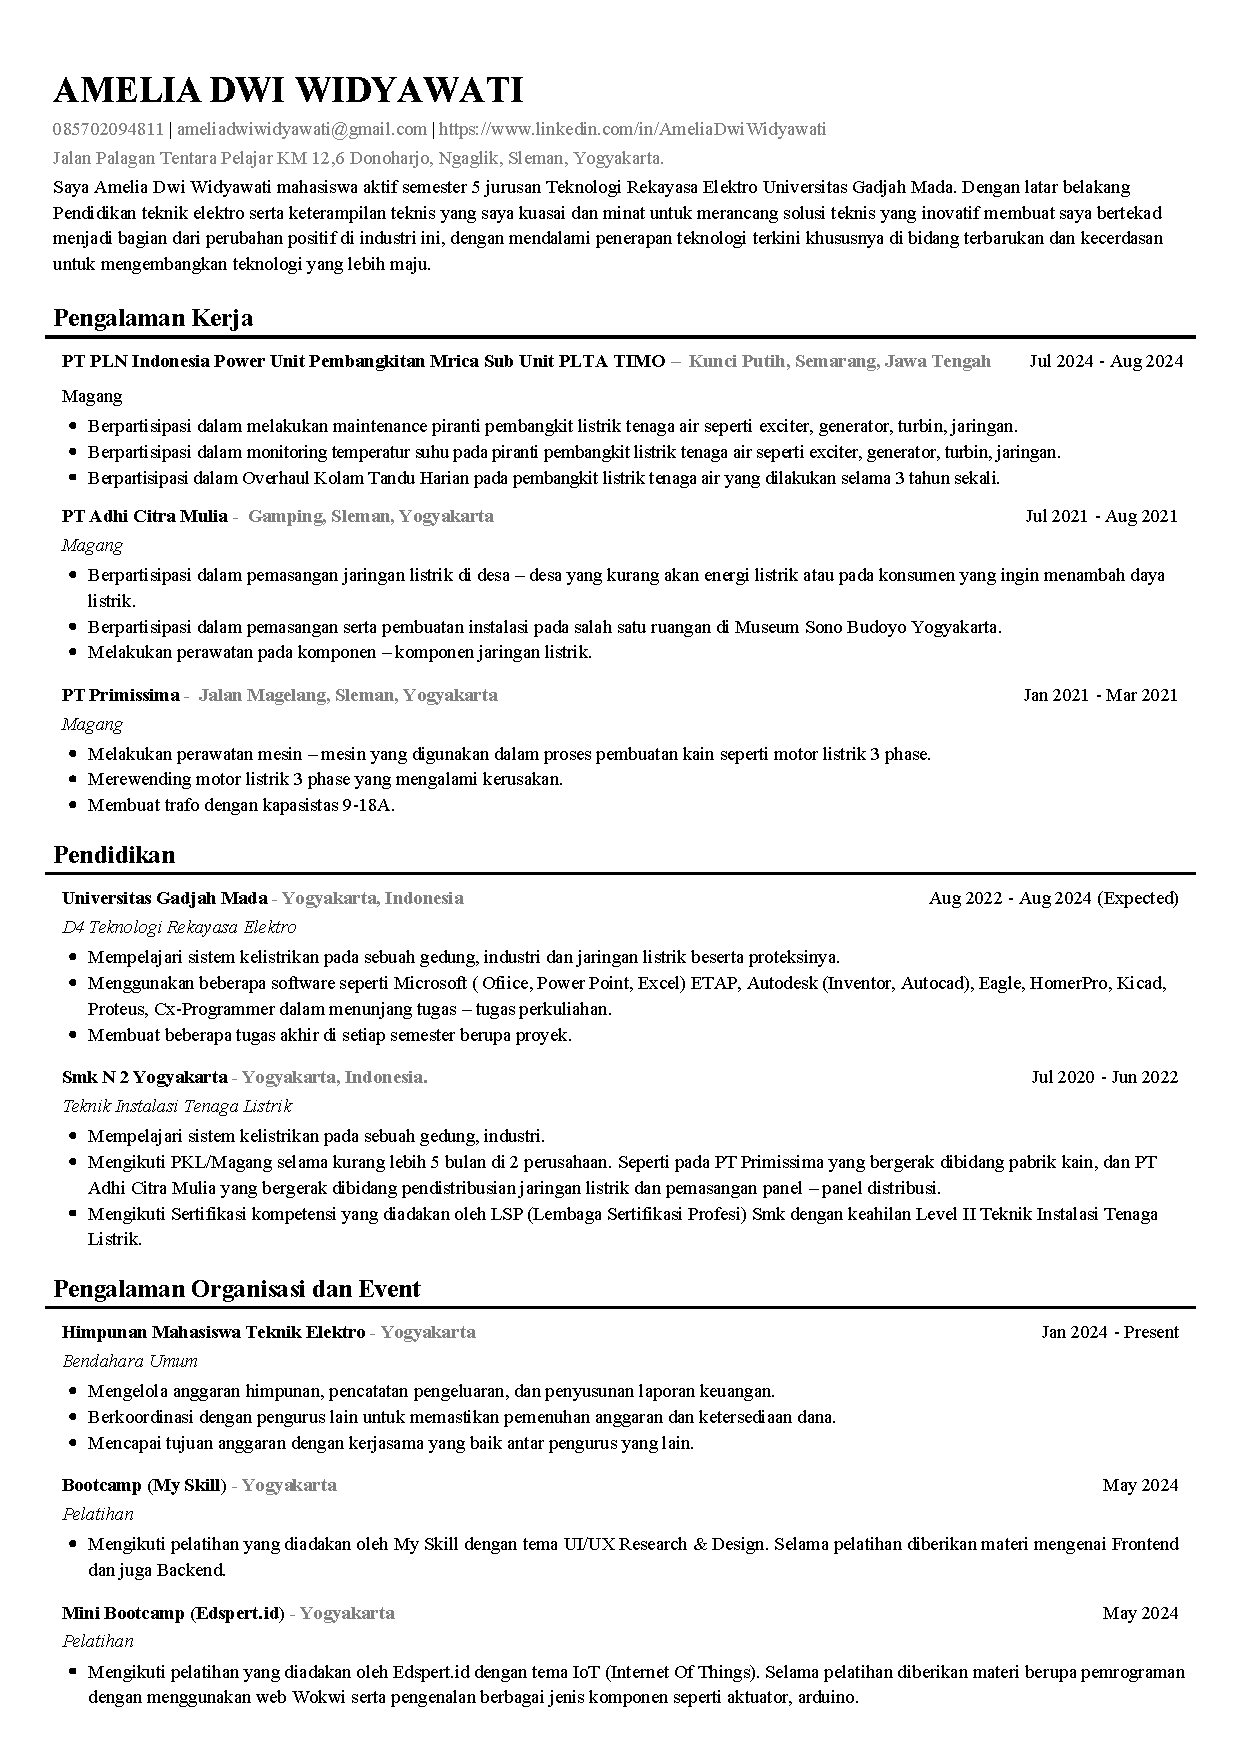
\includegraphics[scale=0.69,page=1]{dokumen/cv_amelia.pdf}
	\newpage
	\includegraphics[scale=0.69,page=2]{dokumen/cv_amelia.pdf}
	
	\newpage		
	\item Transkrip Nilai\\
	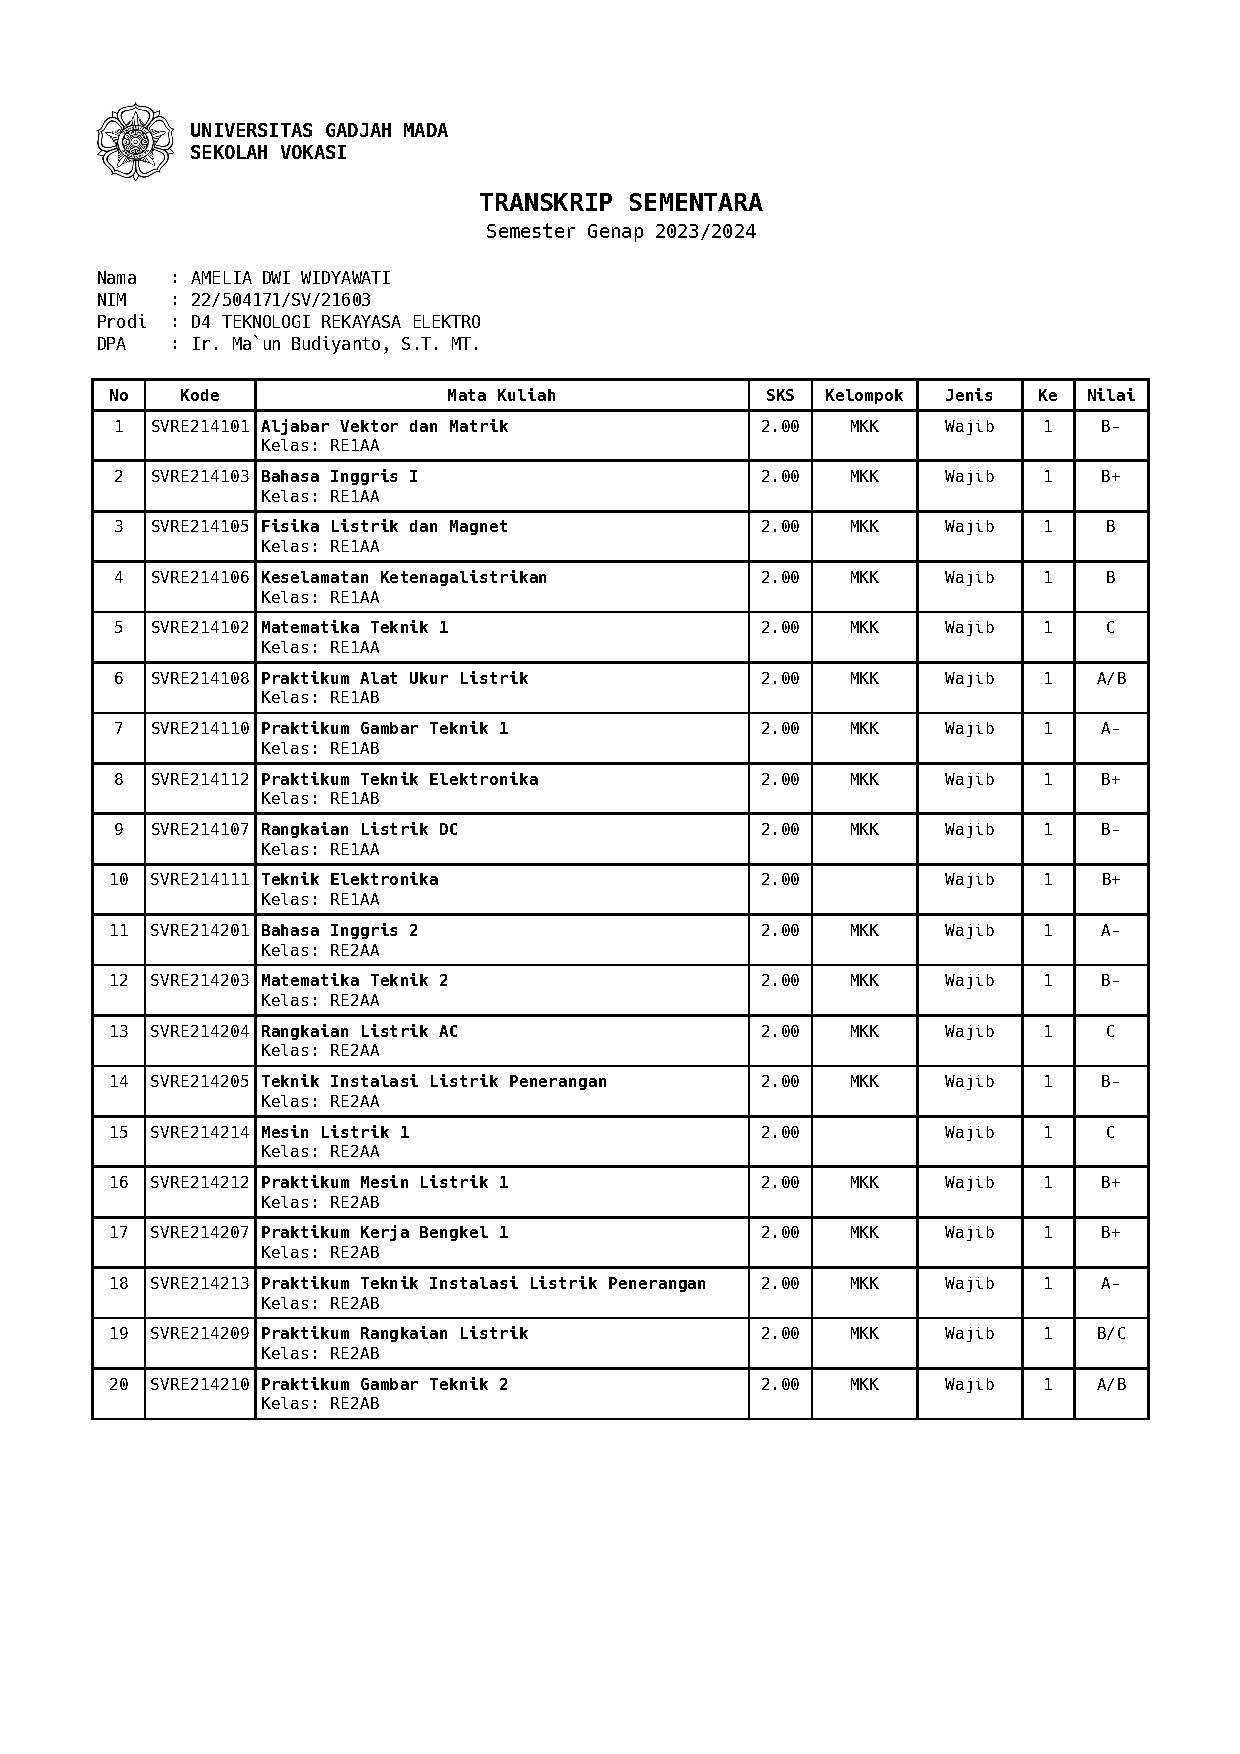
\includegraphics[scale=0.7,page=1]{dokumen/transkrip_amelia.pdf}
	\newpage
	\includegraphics[scale=0.7,page=2]{dokumen/transkrip_amelia.pdf}
	\newpage
	\includegraphics[scale=0.7,page=3]{dokumen/transkrip_amelia.pdf}
	\newpage
	\item Identitas Diri\\ [0.5cm]
	
\includegraphics[scale=0.7]{dokumen/identitas.jpg}
	
	
\end{itemize}



\section{Data Diri {\penulisKedua}}
\begin{itemize}
	
	
	
	\item Riwayat Diri\\
	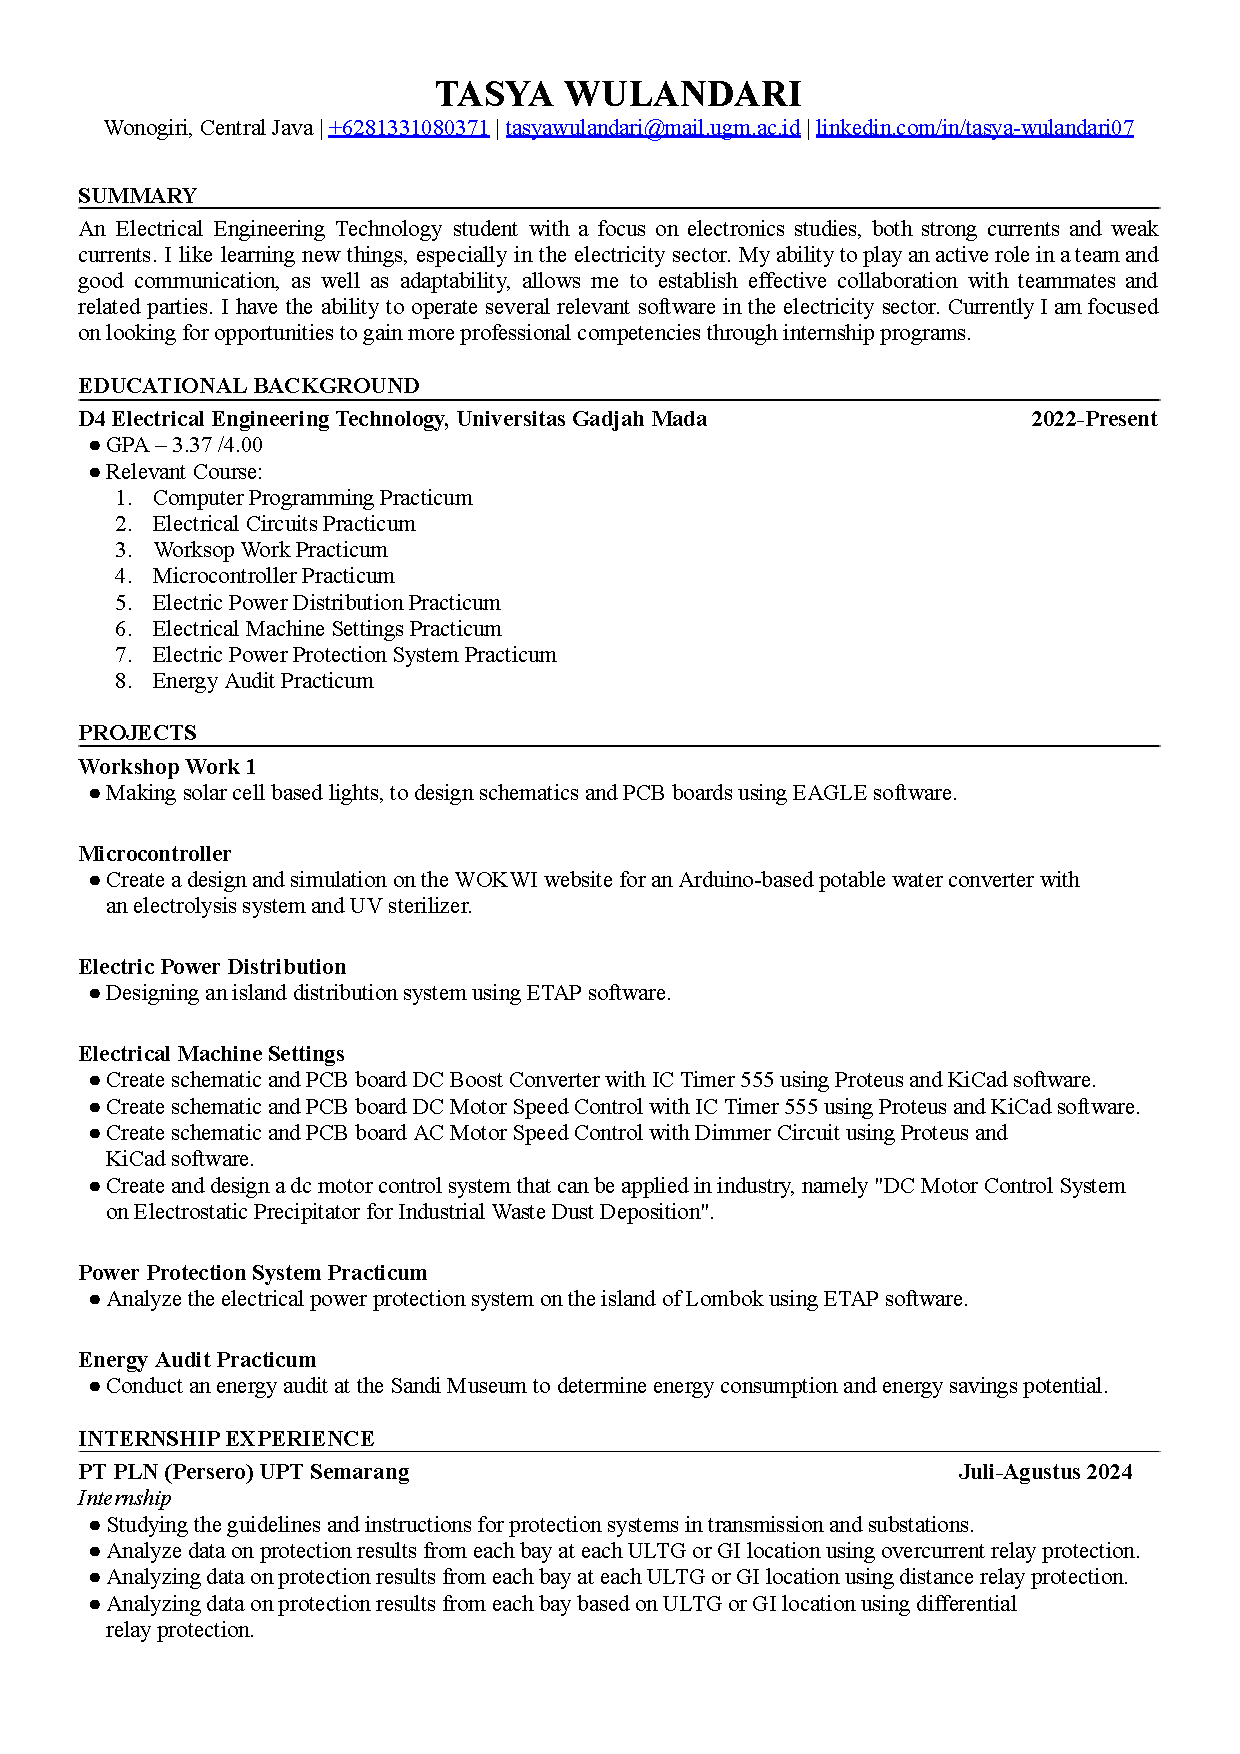
\includegraphics[scale=0.7,page=1]{dokumen/cv_tasya.pdf}
	\newpage
	\includegraphics[scale=0.7,page=2]{dokumen/cv_tasya.pdf}
	
	\newpage		
	\item Transkrip Nilai\\
	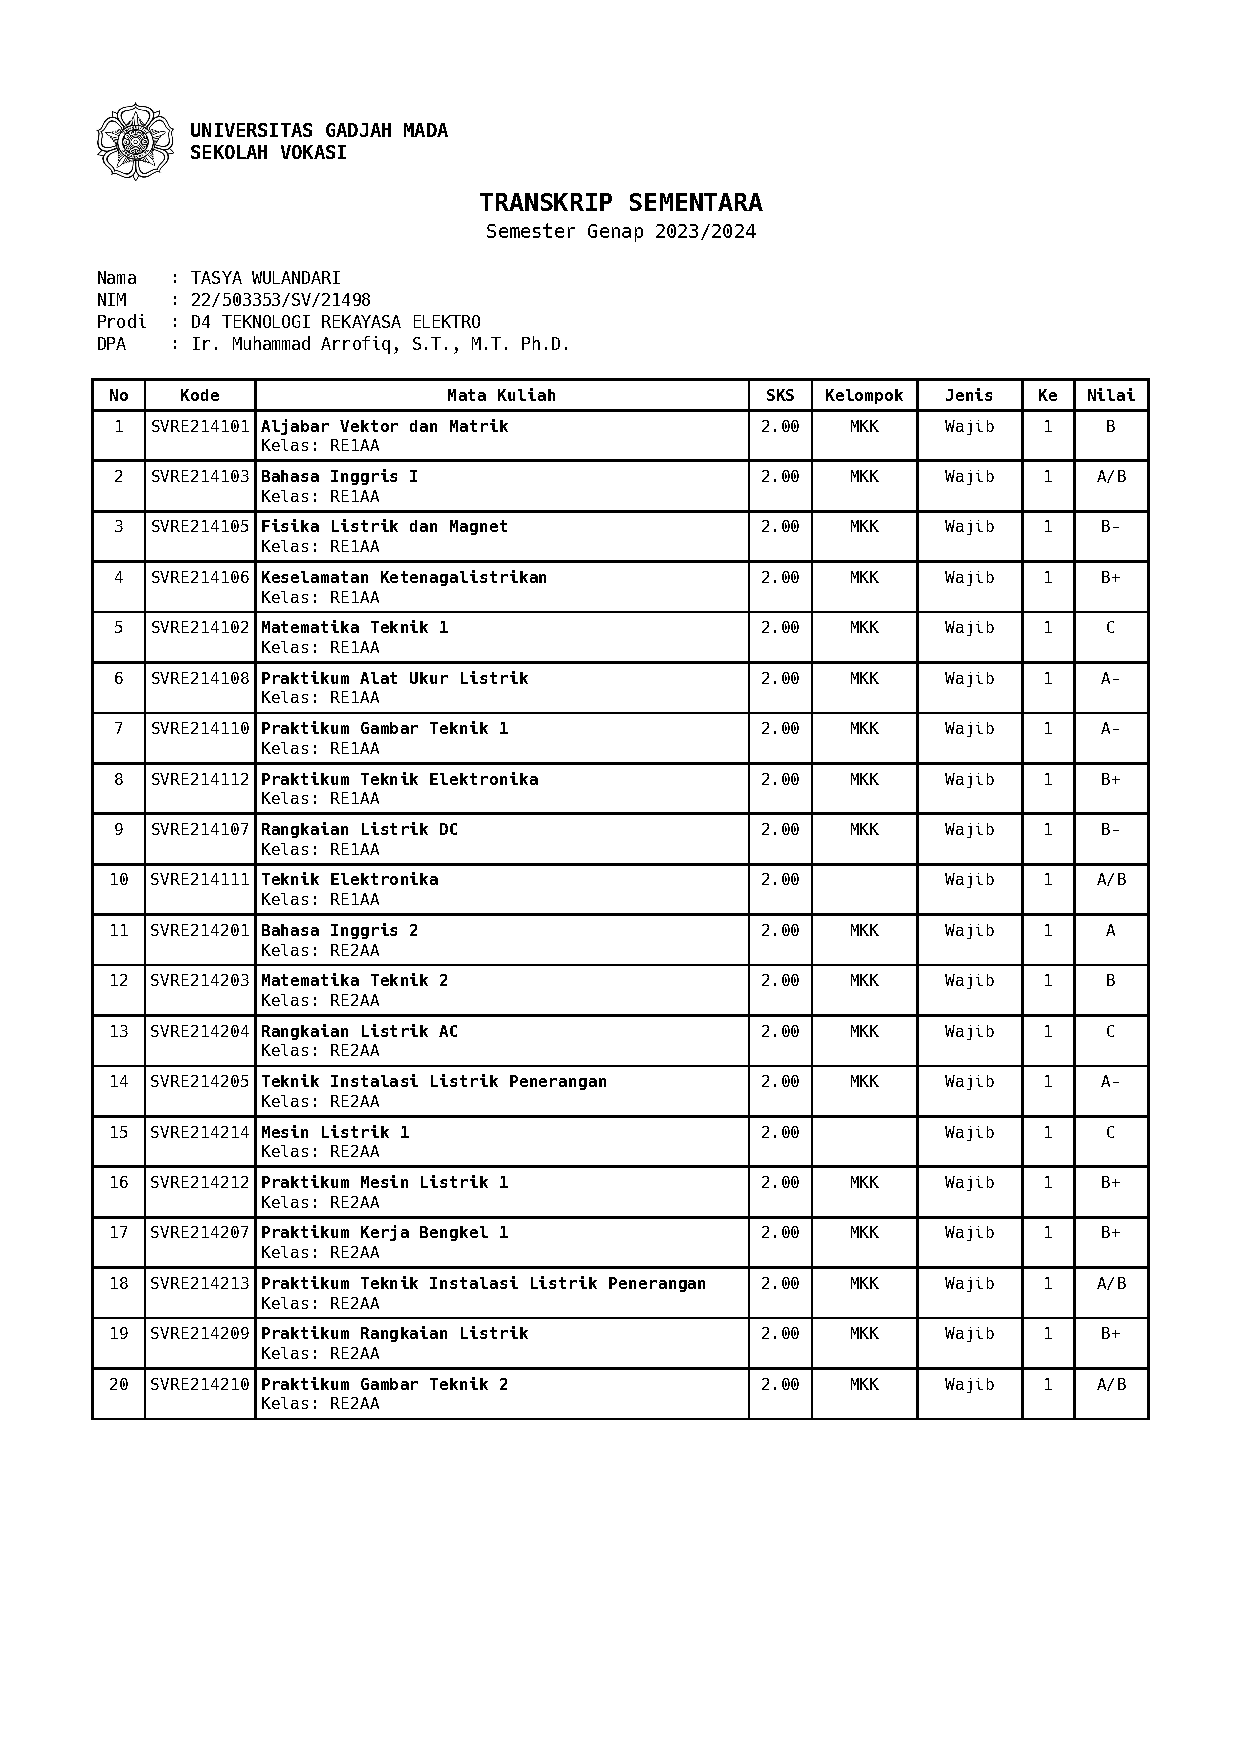
\includegraphics[scale=0.7,page=1]{dokumen/transkrip_tasya.pdf}
	\newpage
	\includegraphics[scale=0.7,page=2]{dokumen/transkrip_tasya.pdf}
	\newpage
	\includegraphics[scale=0.7,page=3]{dokumen/transkrip_tasya.pdf}
	\newpage
	\item Identitas Diri\\ [0.5cm]
	
\includegraphics[scale=0.7]{dokumen/identitas.jpg}
	
\end{itemize}

\end{document}

